%% LyX 2.4.4 created this file.  For more info, see https://www.lyx.org/.
%% Do not edit unless you really know what you are doing.
\documentclass[english]{article}
\usepackage[T1]{fontenc}
\usepackage[latin9]{inputenc}
\usepackage{enumitem}
\usepackage{amsmath}
\usepackage{amsthm}
\usepackage{cancel}
\usepackage{geometry}
\geometry{verbose,tmargin=1in,bmargin=1in,lmargin=1in,rmargin=1in}

\makeatletter
%%%%%%%%%%%%%%%%%%%%%%%%%%%%%% Textclass specific LaTeX commands.
\numberwithin{equation}{section}
\numberwithin{figure}{section}
\newlength{\lyxlabelwidth}      % auxiliary length 

%%%%%%%%%%%%%%%%%%%%%%%%%%%%%% User specified LaTeX commands.
\usepackage{fancyhdr}
\usepackage{lastpage}
\pagestyle{fancy}
\usepackage{enumitem}
\usepackage{ifthen}
%sets math fonts to be more readable
\everymath=\expandafter{\the\everymath\displaystyle}
%\DeclareMathSizes{10}{10}{10}{10}
\usepackage{multicol}

\usepackage{tikz}
\usetikzlibrary{plotmarks}
\usepackage{pgfplots}
\pgfplotsset{compat=newest}

\usepackage{calc}
\usepackage[nomessages]{fp}

\usepackage{advdate}    % Advancing/saving dates
\usepackage{datetime}   % Dates formatting
\usepackage{datenumber} % Counters for dates
% Added by lyx2lyx
\setlength{\parskip}{\smallskipamount}
\setlength{\parindent}{0pt}

\makeatother

\usepackage{babel}
\begin{document}
\renewcommand{\author}{Dr.\,James Ashe}

\newcommand{\classNum}{131}

\newcommand{\classSec}{B}

\newcommand{\nameType}{Name:}

\newcommand{\examType}{Worksheet 4.1}

\renewcommand{\date}{\formatdate{6}{11}{2013}}

%%First page's header%%%%%%%%%%%%%%%%%%%%%%
\fancypagestyle{firststyle} %%header settings for first pagr
{
	\fancyhead[L]{MTH \classNum{}(\classSec{}) \author{}\\
	\textbf{\examType{}} \date{}}
	\fancyhead[C]{\textbf{\nameType}}
	\setlength{\headsep}{14pt}
}
%%%%%%%%%%%%%%%%%%%%%%%%%%%%%%%%%%%%%%%%%%

%%Next page's header%%%%%%%%%%%%%%%%%%%%%%%
\setlist{nolistsep}
\lhead{\classNum{}(\classSec{})} 
\chead{\textbf{\nameType}} 
\cfoot{\thepage{}~of~\pageref{LastPage}} 
\setlength{\headsep}{5pt} 
%%%%%%%%%%%%%%%%%%%%%%%%%%%%%%%%%%%%%%%%%%%

%%Various settings; see the preamble for other settings%%%%%
%%\setenumerate[0]{leftmargin=12pt,itemindent=0pt,labelwidth=0pt}
\renewcommand{\labelenumi}{\textbf{\arabic{enumi}.}}
\renewcommand{\labelenumii}{\textbf{\alph{enumii}.}}
\thispagestyle{firststyle}
%%%%%%%%%%%%%%%%%%%%%%%%%%%%%%%%%%%%%%%%%%
\newcommand{\xmax}{10}
\newcommand{\xmin}{-10}
\newcommand{\xstep}{0} %must be xmin+n
\newcommand{\ymax}{10}
\newcommand{\ymin}{-10}
\newcommand{\ystep}{0} %must be ymin+n

\newcommand{\xspace}{\vspace{1.2cm}}

\emph{Graph the following exponential functions. Clearly indicate
the y-intercept and at least one other point.}
\begin{enumerate}[resume]
\item $f(x)=4^{x}$
\item $g(x)=\left(\frac{1}{3}\right)^{x}$
\end{enumerate}
\begin{multicols}{2}

\renewcommand{\xmax}{10} \renewcommand{\xstep}{10}
\renewcommand{\ymax}{10} \renewcommand{\ystep}{1}
%%%%%%%
\begin{tikzpicture} 
	\begin{axis}[
		axis x line=middle, axis y line=middle,     		
		xtick={-10,-8,...,10},
		ytick={-10,-8,...,10},
		minor x tick num={1},
		minor y tick num={1},
		%ticks=none,
		%no markers,
		grid=both,
		xlabel={$x$},     
		ylabel={$y$},
		xmin=-\xmax.25,xmax=\xmax.25,
		ymin=-\ymax.25,ymax=\ymax.25,     		
		width=7cm,     		
		height=7cm] 		
	%\addplot[red,very thick,mark=noner,smooth] {4^x}; 
	\end{axis}
\end{tikzpicture}

\renewcommand{\xmax}{5} \renewcommand{\xstep}{1}
\renewcommand{\ymax}{4} \renewcommand{\ystep}{1}
%%%%%%%
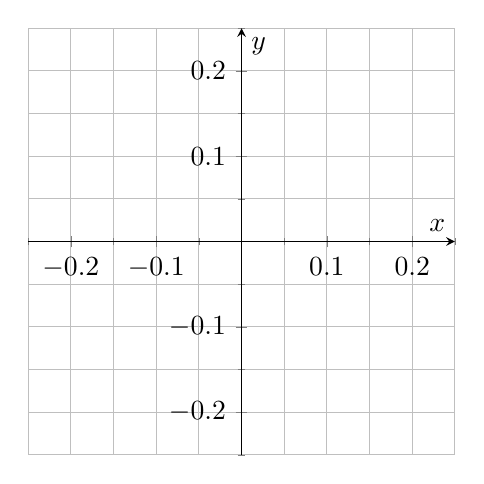
\begin{tikzpicture} 
	\begin{axis}[
		axis x line=middle, axis y line=middle,     		
		%xtick={-\xmax,-\xstep,...,\xmax},
		%ytick={-\ymax,-\ystep,...,\ymax},
		minor x tick num={1},
		minor y tick num={1},
		%ticks=none,
		%no markers,
		grid=both,
		xlabel={$x$},     
		ylabel={$y$},
		xmin=-\xmax.25,xmax=\xmax.25,
		ymin=-\ymax.25,ymax=\ymax.25,     		
		width=7cm,     		
		height=7cm] 		
	%\addplot[red,very thick,mark=noner,smooth] {(1/3)^x}; 
	\end{axis}
\end{tikzpicture}

\end{multicols}
\begin{enumerate}[resume]
\item $f(x)=4^{x}-2$
\item $g(x)=-\left(\frac{1}{3}\right)^{x}$
\end{enumerate}
\begin{multicols}{2}

\renewcommand{\xmax}{10} \renewcommand{\xstep}{10}
\renewcommand{\ymax}{10} \renewcommand{\ystep}{1}
%%%%%%%
\begin{tikzpicture} 
	\begin{axis}[
		axis x line=middle, axis y line=middle,     		
		xtick={-10,-8,...,10},
		ytick={-10,-8,...,10},
		minor x tick num={1},
		minor y tick num={1},
		%ticks=none,
		%no markers,
		grid=both,
		xlabel={$x$},     
		ylabel={$y$},
		xmin=-\xmax.25,xmax=\xmax.25,
		ymin=-\ymax.25,ymax=\ymax.25,     		
		width=7cm,     		
		height=7cm] 		
	%\addplot[red,very thick,mark=noner,smooth] {4^x}; 
	\end{axis}
\end{tikzpicture}

\renewcommand{\xmax}{5} \renewcommand{\xstep}{1}
\renewcommand{\ymax}{4} \renewcommand{\ystep}{1}
%%%%%%%
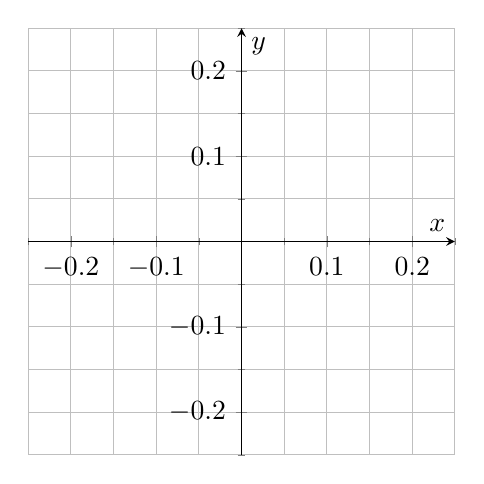
\begin{tikzpicture} 
	\begin{axis}[
		axis x line=middle, axis y line=middle,     		
		%xtick={-\xmax,-\xstep,...,\xmax},
		%ytick={-\ymax,-\ystep,...,\ymax},
		minor x tick num={1},
		minor y tick num={1},
		%ticks=none,
		%no markers,
		grid=both,
		xlabel={$x$},     
		ylabel={$y$},
		xmin=-\xmax.25,xmax=\xmax.25,
		ymin=-\ymax.25,ymax=\ymax.25,     		
		width=7cm,     		
		height=7cm] 		
	%\addplot[red,very thick,mark=noner,smooth] {(1/3)^x}; 
	\end{axis}
\end{tikzpicture}

\end{multicols}
\begin{enumerate}[resume]
\item $f(x)=4^{x+2}$
\item $g(x)=\left(\frac{1}{3}\right)^{x-2}$
\end{enumerate}
\begin{multicols}{2}

\renewcommand{\xmax}{10} \renewcommand{\xstep}{10}
\renewcommand{\ymax}{10} \renewcommand{\ystep}{1}
%%%%%%%
\begin{tikzpicture} 
	\begin{axis}[
		axis x line=middle, axis y line=middle,     		
		xtick={-10,-8,...,10},
		ytick={-10,-8,...,10},
		minor x tick num={1},
		minor y tick num={1},
		%ticks=none,
		%no markers,
		grid=both,
		xlabel={$x$},     
		ylabel={$y$},
		xmin=-\xmax.25,xmax=\xmax.25,
		ymin=-\ymax.25,ymax=\ymax.25,     		
		width=7cm,     		
		height=7cm] 		
	%\addplot[red,very thick,mark=noner,smooth] {4^x}; 
	\end{axis}
\end{tikzpicture}

\renewcommand{\xmax}{5} \renewcommand{\xstep}{1}
\renewcommand{\ymax}{4} \renewcommand{\ystep}{1}
%%%%%%%
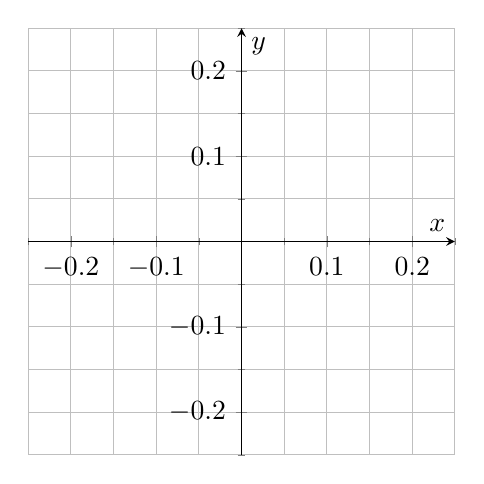
\begin{tikzpicture} 
	\begin{axis}[
		axis x line=middle, axis y line=middle,     		
		%xtick={-\xmax,-\xstep,...,\xmax},
		%ytick={-\ymax,-\ystep,...,\ymax},
		minor x tick num={1},
		minor y tick num={1},
		%ticks=none,
		%no markers,
		grid=both,
		xlabel={$x$},     
		ylabel={$y$},
		xmin=-\xmax.25,xmax=\xmax.25,
		ymin=-\ymax.25,ymax=\ymax.25,     		
		width=7cm,     		
		height=7cm] 		
	%\addplot[red,very thick,mark=noner,smooth] {(1/3)^x}; 
	\end{axis}
\end{tikzpicture}

\end{multicols}
\end{document}
